\chapter{Resultados}\label{ch:resultados}


\section{Resultados relativos al objetivo 1}\label{sec:resultados-relativos-al-objetivo-1}

Los resultados de este objetivo corresponden con la selección de
tecnologías adecuadas para el desarrollo de la aplicación,
eligiendo un lenguaje de programación y un \textit{framework} de
desarrollo de aplicaciones de escritorio que permitan crear
aplicaciones modernas, multiplataforma, de gran calidad,
y que permitan cargar código externo a voluntad.

El proceso de búsqueda y selección del lenguaje de programación y
del framework culminó con la elección de \textit{Java 17}
y \textit{JavaFX} respectivamente.
Con estas tecnologías se ha conseguido desarrollar una aplicación
moderna y multiplataforma, con soporte para componentes y totalmente
personalizable.

Gracias al uso de una versión de \textit{Java} moderna,
el desarrollo de la aplicación ha sido \textbf{muy rápido} y el resultado
ha sido \textbf{muy profesional}, pudiendo implementar diseños y
algoritmos rápidamente y con pocos errores.
\textit{JavaFX} ha permitido desarrollar una interfaz de usuario
que se separa del conocido y desfasado formato de las aplicaciones
\textit{Swing}.
Gracias a su fácil desarrollo y su capacidad de usar código
\textit{CSS} para definir el estilo de la aplicación, \textit{JAMS}
cuenta con un aspecto moderno y profesional.

Una de las ventajas que ha aparecido durante el
desarrollo gracias a utilizar \textit{Java} ha sido la
capacidad de poder usar otros lenguajes de programación capaces
de compilar a la \textit{JVM} para el desarrollo de componentes.
Así, el desarrollador podrá escoger entre un \textbf{amplio abanico de lenguajes}
de programación para crear su componente.
Algunos ejemplos de lenguajes de programación que compilan a la \textit{JVM}
son \textit{Scala}, \textit{Kotlin} o \textit{Groovy}.
Un ejemplo de componente desarrollado en \textit{Kotlin} sería
\textit{NES4JAMS}, que forma parte del Trabajo de Fin de Grado
realizado por el autor para la obtención del título de Grado en
Diseño y Desarrollo de Videojuegos.

\section{Resultados relativos al objetivo 2}\label{sec:resultados-relativos-al-objetivo-2}

Los resultados de este objetivo corresponden con la creación de
un entorno base y un \textit{framework} que permita \textbf{implementar
diferentes entornos y herramientas}, creando así una capa
de abstracción que ayuda a los desarrolladores y al propio
\textit{JAMS} a crear herramientas de manera rápida y sencilla.

Se considera que este objetivo se ha conseguido.
Gracias a las diferentes tecnologías que se han desarrollado
para la base, es posible crear nuevas herramientas en cuestión
de minutos.

Los requisitos establecidos en el Trabajo Fin de Grado del Grado en Diseño
y Desarrollo de Videojuegos de la misma autoría y que se apoya en el presente
trabajo han motivado la necesidad de introducir cambios y mejoras en el código
que han contribuido a que \textit{JAMS} actualmente se haya convertido en una
aplicación base robusta, con capacidad de personalizar
una gran cantidad de aspectos del entorno.

La base también permite a los usuarios más comunes e
inexpertos personalizar el entorno de desarrollo gracias a la
\textbf{extensa configuración} y la capacidad de poder producir
\textbf{paquetes de idiomas y de temas}.
El resultado de estas personalizaciones se puede apreciar
perfectamente en la figura \ref{fig:jams-collage}.

\begin{figure}[h]
    \centering
    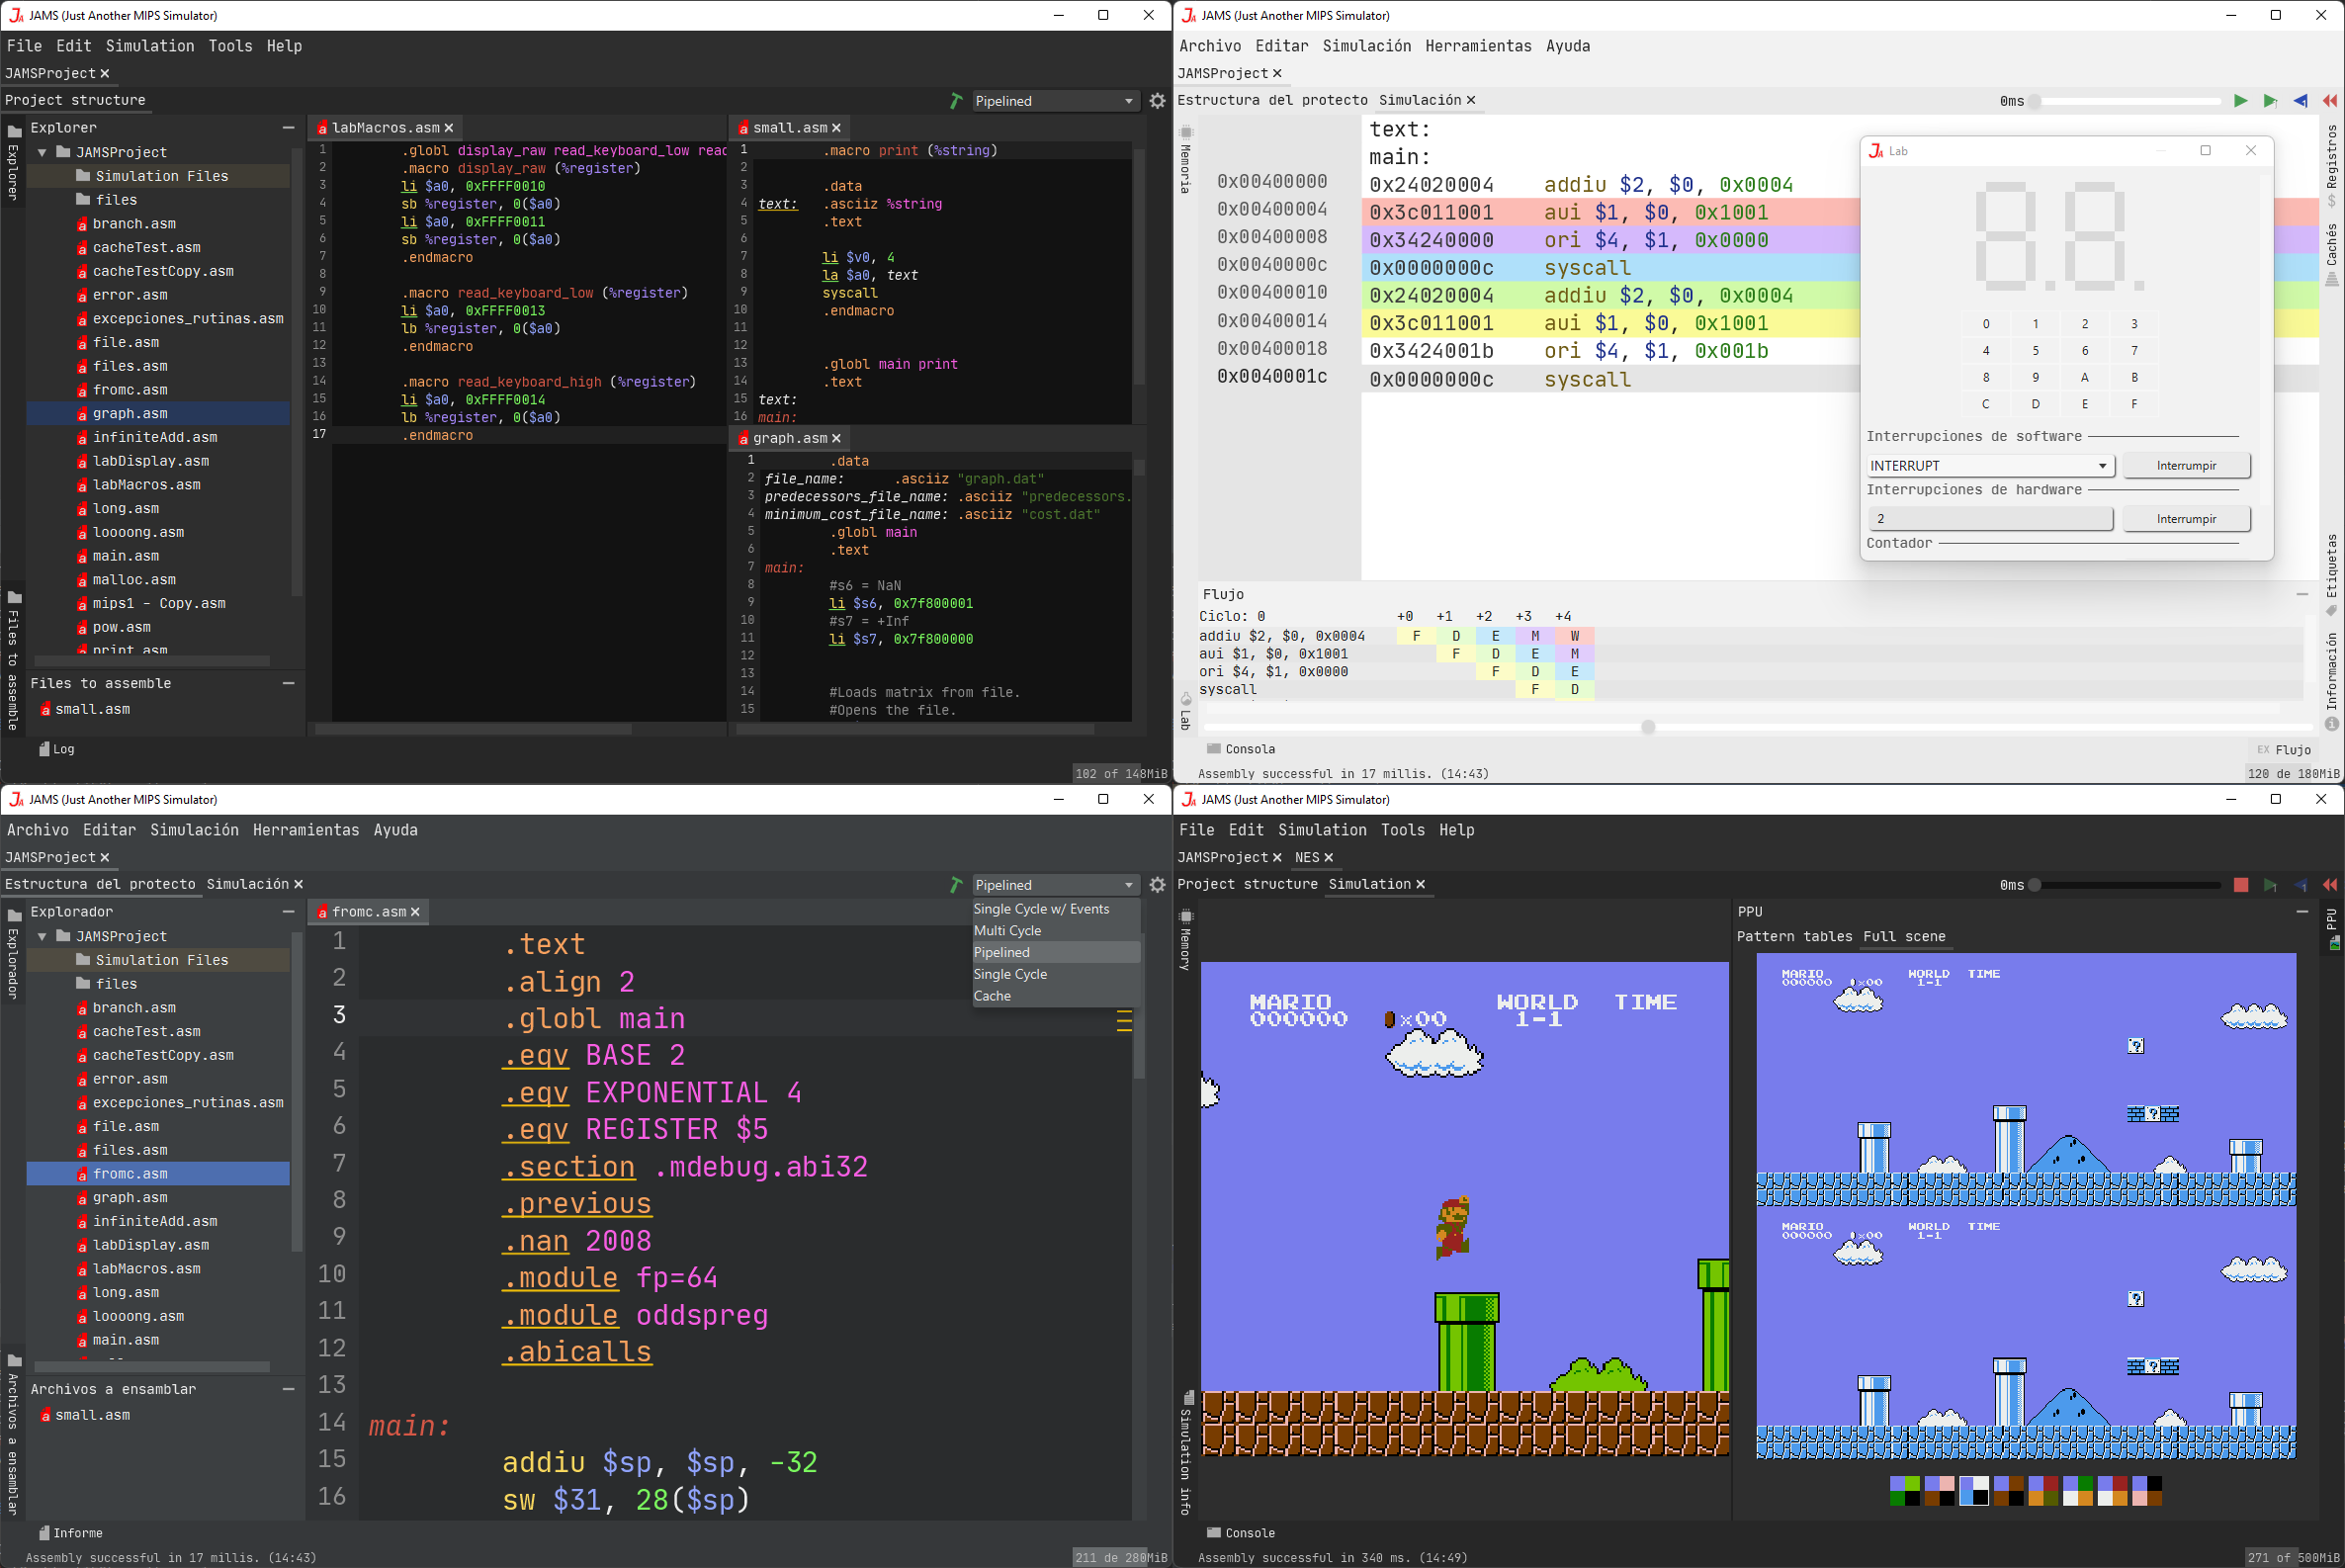
\includegraphics[width=0.8\textwidth]{images/result/jams-collage}
    \caption{Diferentes perfiles de personalización de \textit{JAMS}}
    \label{fig:jams-collage}
\end{figure}

Por último, destacar el resultado de la \textit{interfaz de usuario}.
El uso de nodos como elemento central de la interfaz puede considerarse
un \textbf{acierto}: son componentes muy fáciles de usar y altamente personalizables.
Estos nodos son independientes entre sí, y muchos de ellos son \textbf{independientes}
de la tecnología empleada por el usuario, como es el caso del \textbf{explorador}.
Esto permite que sean herramientas \textbf{altamente reutilizables}, estando en todo
momento a disposición del desarrollador de componentes.


\section{Resultados relativos al objetivo 3}\label{sec:resultados-relativos-al-objetivo-3}

Los resultados de este objetivo corresponden con la implementación
de un entorno de desarrollo para la arquitectura \textit{MIPS32}
usando la base creada en el objetivo anterior.
El objetivo requiere de la creación de un editor, un ensamblador
y un simulador, además de diferentes herramientas que complementen
a estos tres elementos principales.

Se considera que este objetivo se ha superado
de manera óptima.
\textit{JAMS} presenta de inicio un entorno de desarrollo completo
para la arquitectura \textit{MIPS32}.

El \textbf{editor de texto} está al nivel de los editores de texto
inteligentes que se pueden encontrar en los entornos de desarrollo
actuales, \textbf{ayudando al usuario} en la mayoría de las tareas
relacionadas con la programación de una aplicación en ensamblador, como se observa
en la figura \ref{fig:mips-editor}.

\begin{figure}[ht]
    \centering
    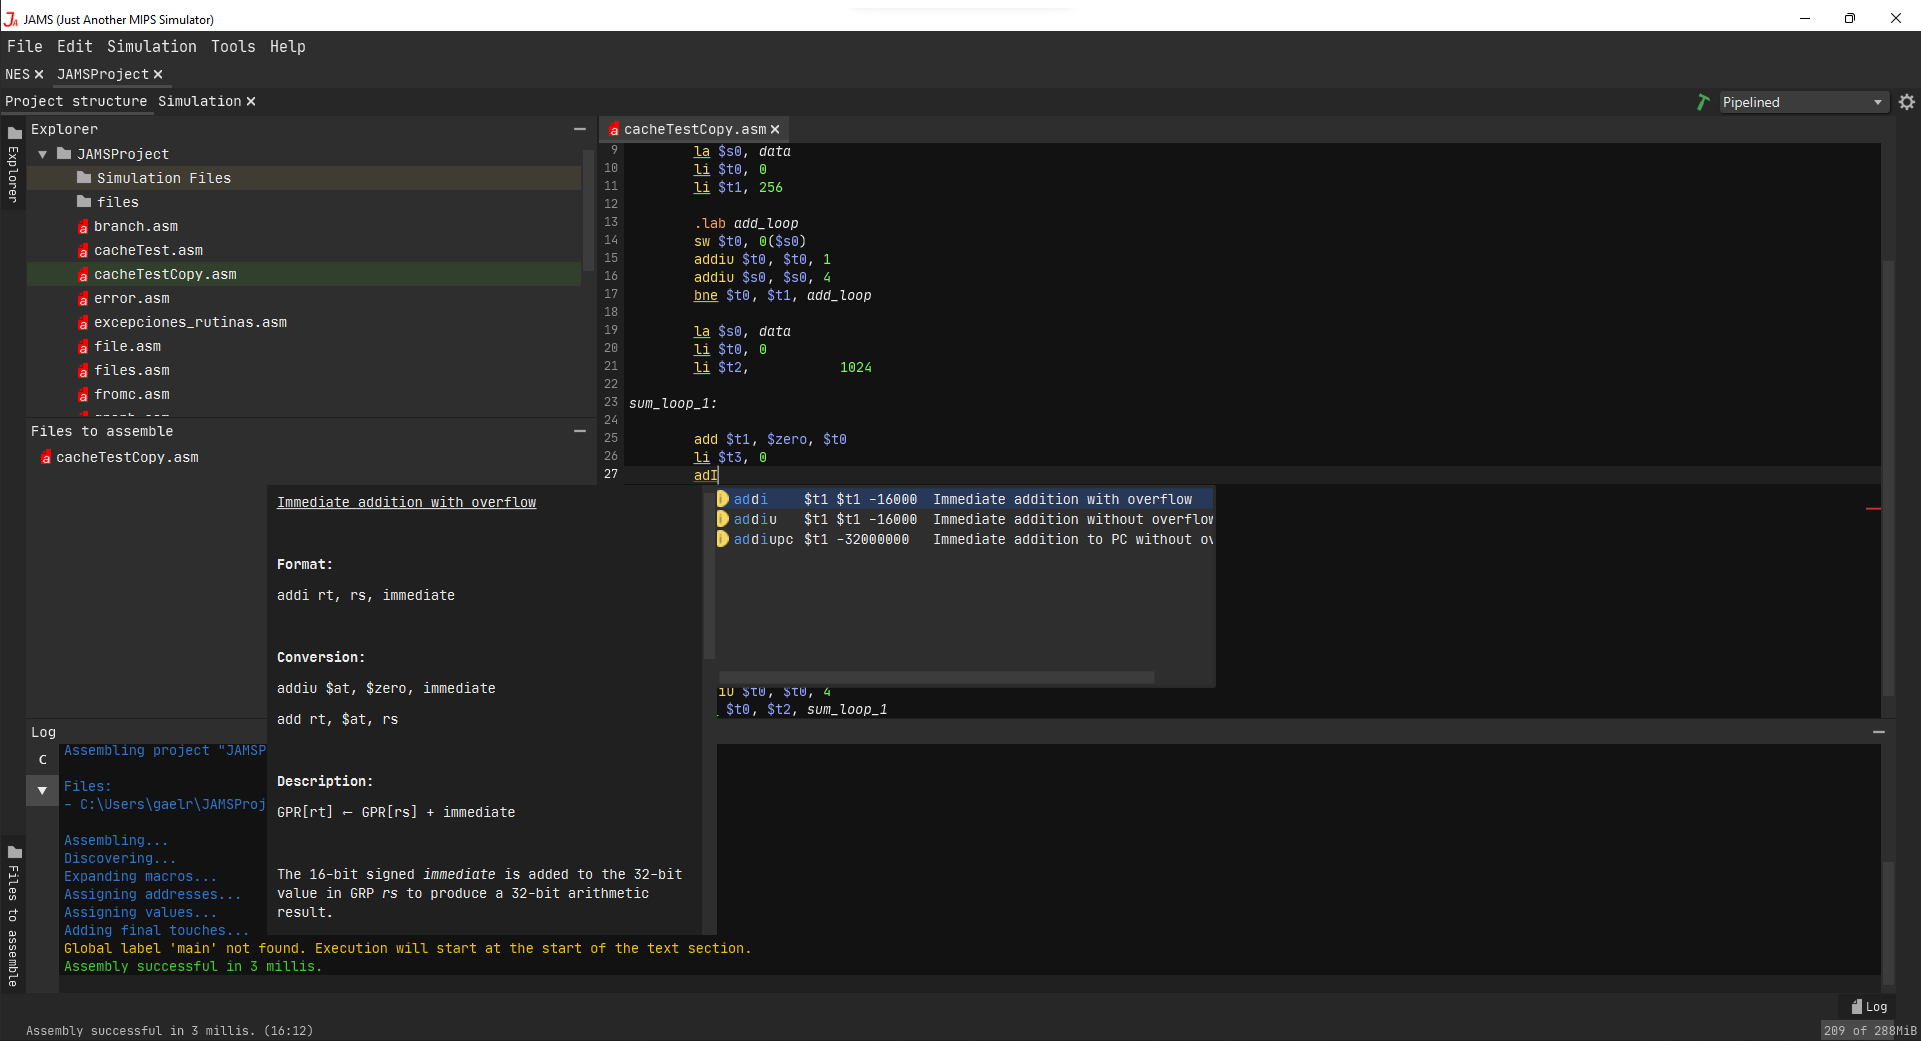
\includegraphics[width=\textwidth]{images/result/mips-editor}
    \caption{Editor de texto proporcionando ayuda al usuario}
    \label{fig:mips-editor}
\end{figure}

El \textbf{ensamblador} es altamente \textbf{personalizable},
permitiendo que otros componentes puedan aportar nuevas instrucciones y
directivas de manera sencilla.
Este ensamblador también incorpora varias \textbf{características avanzadas}
que el usuario puede emplear, como son las \textbf{macros} y las
\textbf{etiquetas relativas}.

El \textbf{simulador} permite ejecutar código ensamblador
\textbf{MIPS32} en diferentes arquitecturas, siendo la arquitectura
uniciclo la más rápida de todas ellas, llegando a superar los
\textbf{40 millones de ciclos cada segundo}.
El simulador está equipado con diversas herramientas que
permiten al usuario \textbf{visualizar y modificar} su estado
de diversas maneras, tal y como se puede observar en la figura \ref{fig:mips-tools}.
Como detalle final, el simulador presenta una estructura basada en
\textbf{hilos}, lo que evita que \textit{JAMS} se congele al ejecutar
una aplicación.

\begin{figure}[!t]
    \centering
    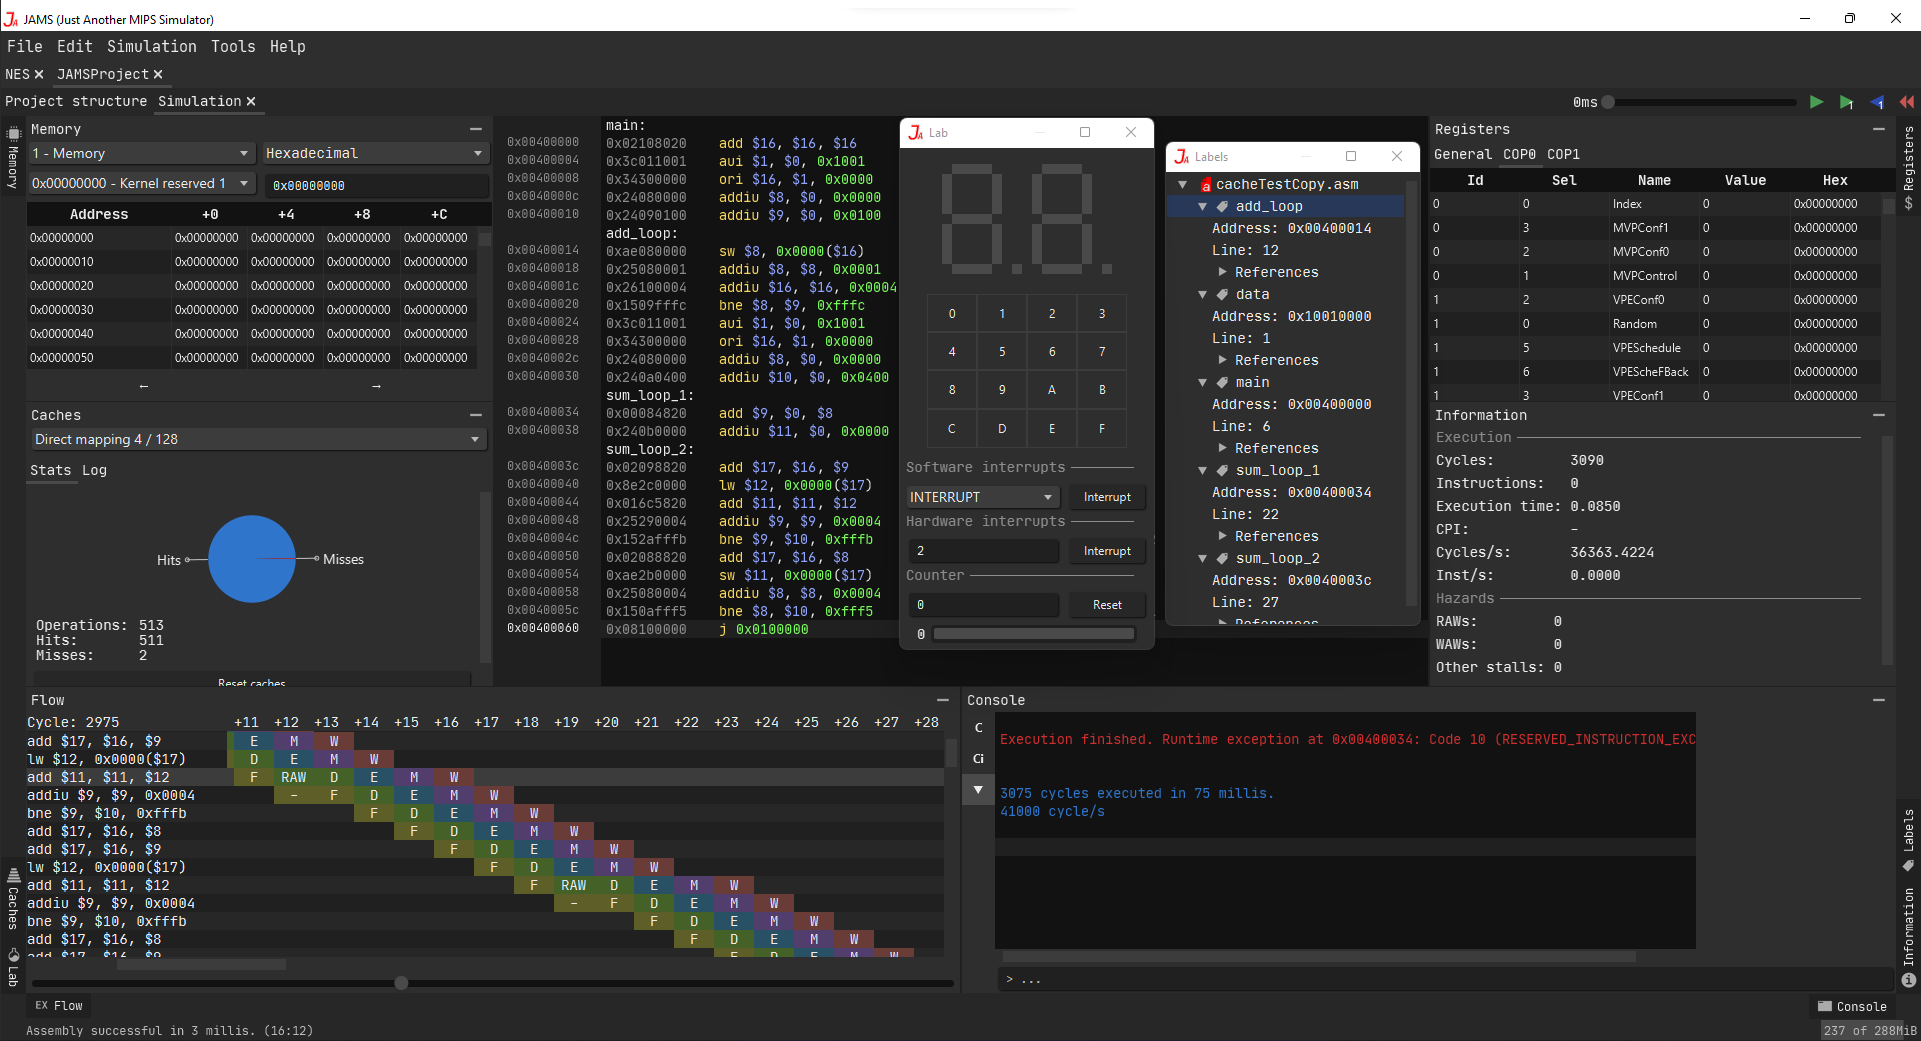
\includegraphics[width=\textwidth]{images/result/mips-tools}
    \caption{Todas las herramientas proporcionadas por el simulador}
    \label{fig:mips-tools}
    \vspace{12cm}
\end{figure}
